\documentclass[a4paper, 12pt]{article}
\usepackage{comment} % enables the use of multi-line comments (\ifx \fi)
\usepackage{graphicx}
\usepackage{fullpage} % changes the margin
\usepackage{listings}
\usepackage{xparse}
\usepackage{xcolor}
\usepackage{minted}
\usepackage{amsmath}
\usepackage{varwidth}
\usepackage{tikz}

\usetikzlibrary{shapes,arrows,automata}

\tikzstyle{block} = [draw, fill=blue!20, rectangle, 
    minimum height=3em, minimum width=6em]
\tikzstyle{sum} = [draw, fill=blue!20, circle, node distance=1cm]
\tikzstyle{input} = [coordinate]
\tikzstyle{output} = [coordinate]
\tikzstyle{pinstyle} = [pin edge={to-,thin,black}]

\NewDocumentCommand{\codeword}{v}{%
\texttt{\textcolor{blue}{#1}}%
}

\newcommand{\block}[1]{%
  \begingroup
  \setlength{\fboxsep}{0pt}%
  \vrule width0pt height \blockdim
  \ooalign{%
    \framebox[\blockdim]{\rule{0pt}{\blockdim}}\cr
    \hidewidth\raisebox{0.5\dimexpr\blockdim-\height}{\raisebox{\depth}{#1}}\hidewidth\cr
  }%
  \endgroup
}
\newcommand{\joinblocks}{\unskip\kern-\fboxrule\ignorespaces}
\newenvironment{blocks}[1][1cm]
 {\begin{varwidth}{\textwidth}\setlength{\blockdim}{#1}\makeblocks}
 {\end{varwidth}}
\newcommand{\makeblocks}{%
  \begingroup\lccode`~=`&\lowercase{\endgroup\let~}\joinblocks
  \catcode`\&=\active
  \baselineskip=0pt
  \lineskiplimit=\maxdimen
  \lineskip=0pt
  \centering
}
\newlength{\blockdim}

\begin{document}
% Header
\noindent
\LARGE\textbf{Intrastellar} \hfill \\
\newline
\large\textbf{Preliminary Design Report} \hfill \textbf{Zach Schuermann} \\
\normalsize ECE 4273-001 \hfill 112944063 \\
Dr. Erik Petrich \hfill Date: 04/16/19 

\section*{Project Objectives}
The ultimate goal for this project is to create a Galaga-like game implemented on an LPC1769 with a Playstation 2 controller for user input/control and a 480x800 LCD display.

\section*{Solution Design}
add more

\begin{center}
  \begin{tabular}{ |c|c|c| }
    \hline
    \textbf{Component} & \textbf{Description} & \textbf{Points} \\
    \hline
    \hline
    Game Type & Animated real-time game (objects continuously in motion) & 2 \\
    \hline
    Display & Use a graphical LCD for output  & 2 \\
    \hline
    Input & Use a game controller with a serial interface (Playstation 2) & 0.5 \\ 
    \hline
    Sound & Use D-to-A to generate a sine wave based sound effect  & 1 \\
    \hline
    Other & Use non-volatile memory (EEPROM  to retain high score table) & 0.5 \\ 
    \hline
    Total & & 6 \\ 
    \hline
  \end{tabular}
\end{center}

\section*{Hardware Design}

\begin{figure}[h!]
  \centering
  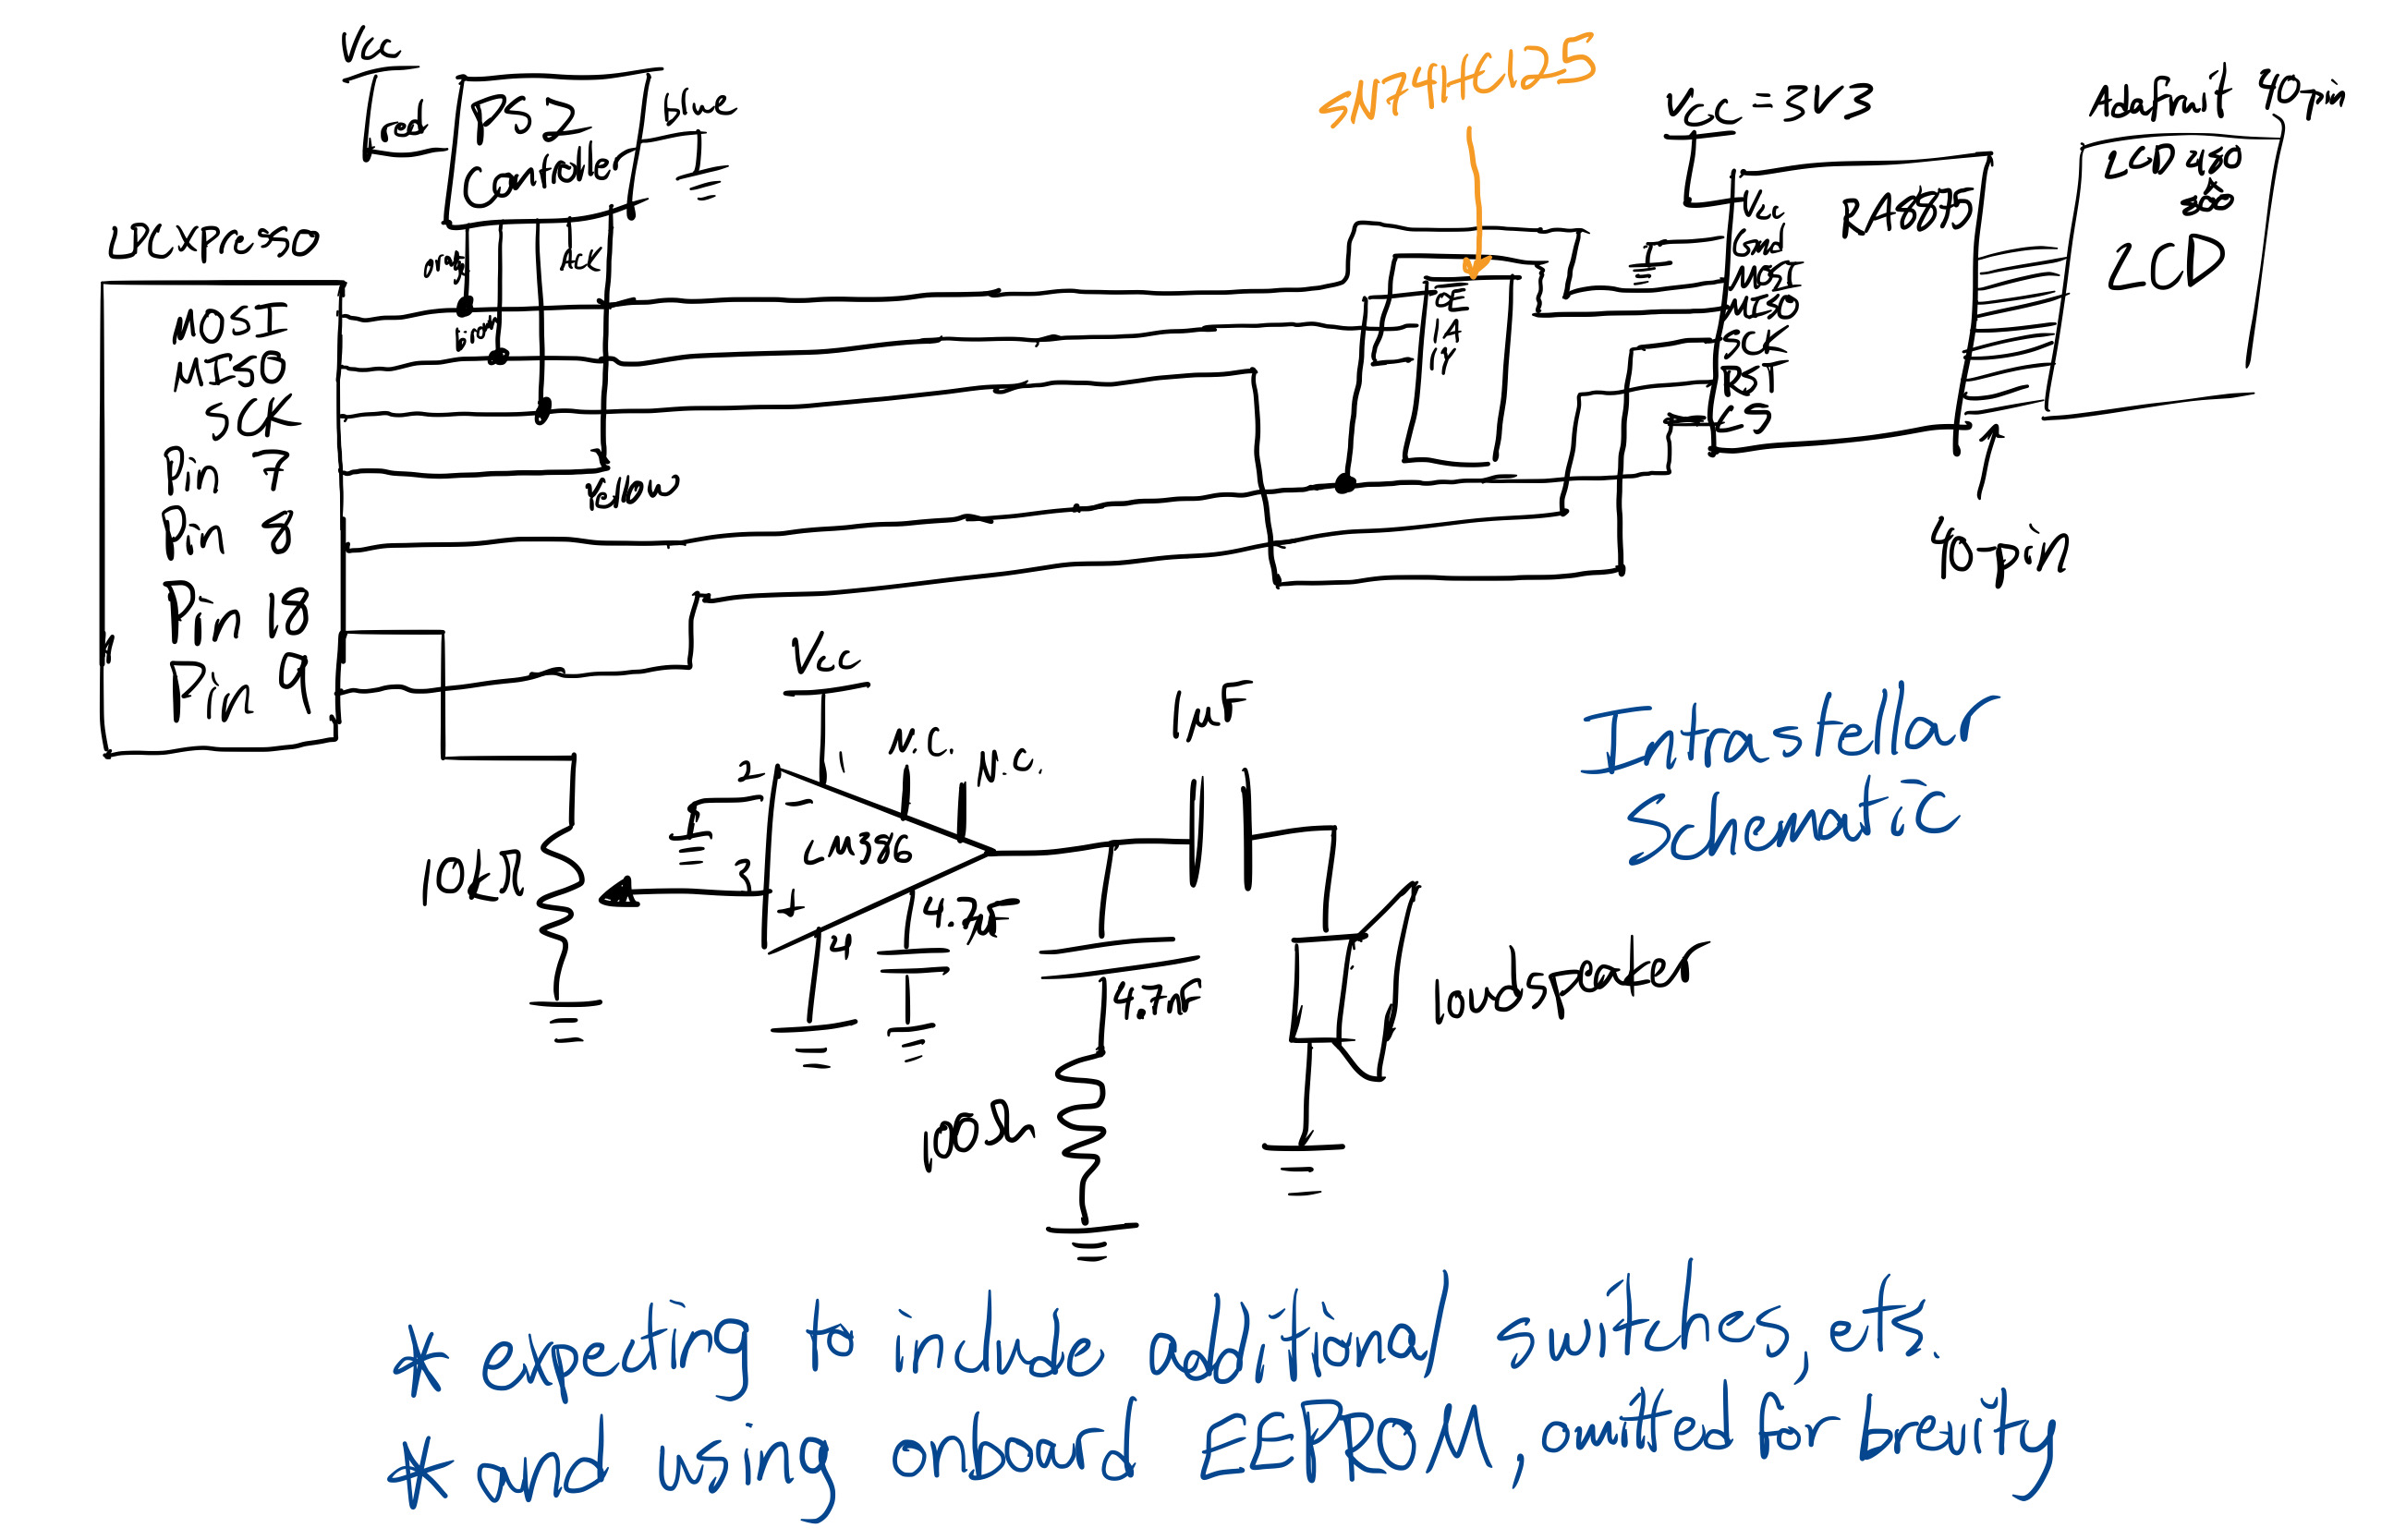
\includegraphics[scale=.6]{schematic.png}
  \caption{Preliminary Hardware Schematic}
  \label{fig:schematic}
\end{figure}

schematic in Figure \ref{fig:schematic}


\section*{Software Design}
The software

%\begin{minted}{c}
%\end{minted}
%\section*{Discussion}

\end{document}
